\documentclass{article}
    \usepackage{url}
    \usepackage{cite}
    \usepackage{float}   
    \usepackage{xcolor}
    \usepackage{lscape}
    \usepackage{amssymb}
    \usepackage{titling}
    \usepackage{pdfpages}
    \usepackage{enumitem}
    \usepackage{graphicx}
    \usepackage{hyperref}
    \usepackage{fancybox}
    \usepackage{enumerate}
    \usepackage{pdflscape}
    \usepackage{afterpage}
    \usepackage{listingsutf8}
    \usepackage[margin=0.8in]{geometry}
    \usepackage[nottoc,notlot,notlof]{tocbibind}
    \renewcommand\maketitlehookd{\vfill\null}
    \renewcommand\maketitlehooka{\null\mbox{}\vfill}

    \newcommand\backgroundimage{
        \put(-5,0){
        \parbox[b][\paperheight]{\paperwidth}{
        \vfill
        \centering
        
\includegraphics[height=\paperheight]{Images/background.jpg}
        \vfill
    }}}

    \newcounter{num}

    \graphicspath{ {Images/} }

    \title{EBUS3030 Assignment 1}
    \author{
        Steven Karmaniolos 
        \texttt{c3160280@uon.edu.au}\\
        Jay Rovacsek
        \texttt{c3146220@uon.edu.au}\\
        Jacob Litherland
        \texttt{c3263482@uon.edu.au}\\
        Edward Lonsdale
        \texttt{c3252144@uon.edu.au}
    }
    \date{\today}
    \hypersetup{
    colorlinks=true,
    linkcolor=black,
    filecolor=magenta,      
    urlcolor=blue,
    citecolor=red,
    linktoc=section,
    }
    \pagenumbering{arabic}

    \newlist{legal}{enumerate}{10}
    \setlist[legal]{label*=\arabic*.}

    \begin{document}
    \AddToShipoutPicture{\backgroundimage}

    \begin{titlingpage}
        \maketitle
    \end{titlingpage}

    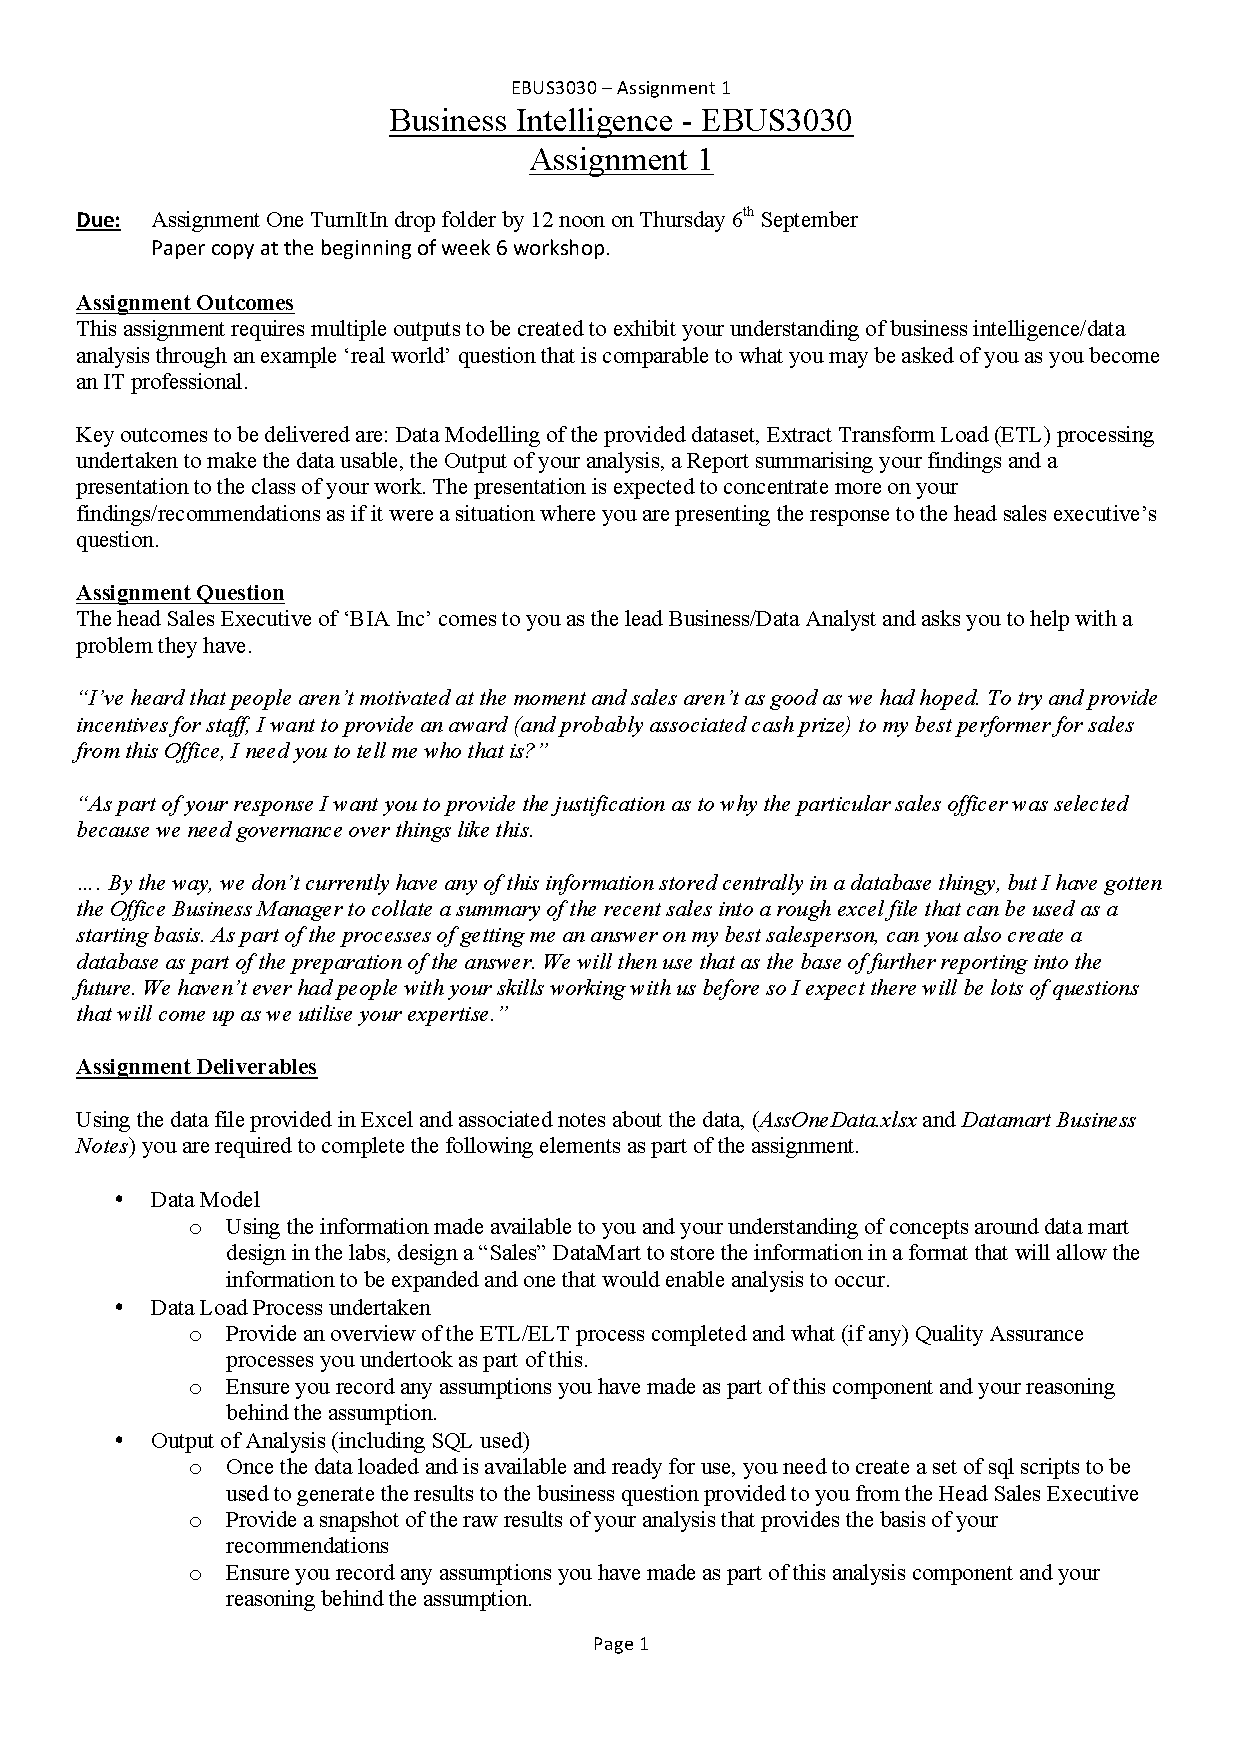
\includepdf[height=\paperheight,keepaspectratio,pages={1,2}]{Resources/Assignment1Overview.pdf}

    \section{Datamart Business Notes}
    The following business rules were provided to be used in the context of this assignment:
    \begin{itemize}
        \renewcommand\labelitemi{*}
        \item At BIA all customers interacts are in an online environment, 
        there are no orders outside of electronic.
        \item Returning customers can provide POI information via the web
        interface and look up their record and that will flow with the sale.
        \item The sales associate can complete the order form/sale for the
        client.
        \item Each sale will have a receipt number/id.
        \item A receipt can have many line items.
        \item Each line item can only be for a single item, but the customer can
        purchase multiples of the same item.
        \item Where a customer has multiple line items, any sale with more than
        5 row items (containing at least 5 different items) is provided a
        15\% discount.
        \item The system automatically handles the total for the sale by looking
        up the item, then multiplying the costs per item by number
        purchased, and then should store this final field total as a record
        in the system (but should also be able to see clearly sales that
        were provided a discount.
        \item Item prices can change at any point, and the price the customer
        pays is the amount listed for the item on the sale date. We need to
        keep a record of all item prices historically.
        \item Only 1 BIA sales assistant can be attributed to any receipt.
    \end{itemize}

    \newpage
    \section{Data Model}
    The below data model is only a suggestion and is still subject to change into the future. A full create script can be found in the \hyperref[sec:Appendix]{\color{blue}appendix}
        \begin{center}
            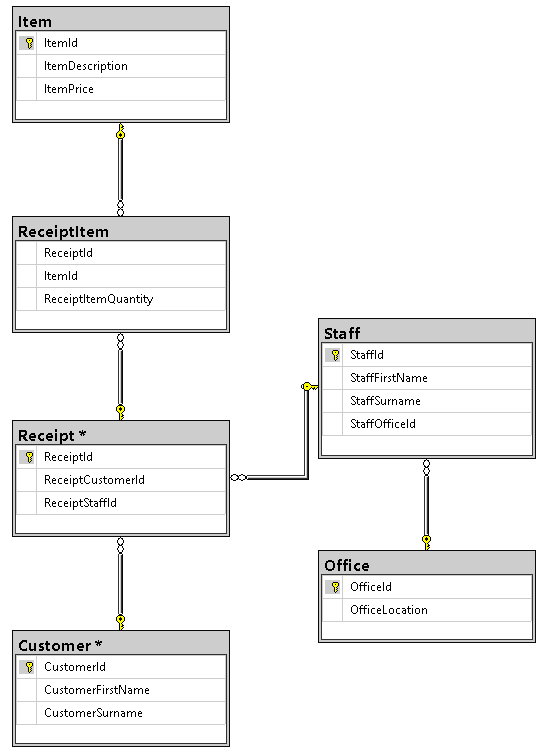
\includegraphics[width=\textwidth]{Images/Suggested_Schema.PNG}
        \end{center}
    It must be noted that the structure of this data model is 
    less than efficient, and it would be expected in a datamart
    situtation that only at lower levels of data would this schema
    remain responsive in the manner it is now, as the outline
    suggests the datamart is not necessarily the most suitable
    design for future use, however suits very well currently.
    \par
    It would be expected that only at extremely large datasets
    would this model prove a bad design. In such cases a model 
    more representative of the snowflake or star schemas would be
    heavily advised.

    \newpage
    \section{Data Load Process (ETL/ELT)}
        Initial import of the data supplied in the xlsx file generated a very basic table
        that allowed us to analyse the data for potential outliers, confirm the business
        requirements of the data and then create tables from which the data model was derived.
        \\
        The Imported table structure was as follows:
        \begin{center}
            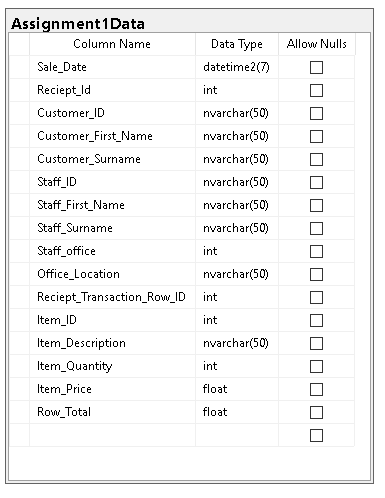
\includegraphics{Images/Initial_Import.PNG}
        \end{center}

        A decision to leave this initial import table as default
        was made to allow easy reference to the initally supplied
        excel data file.
        \par
        In the following sections of \hyperref[sec:QAP]{\color{blue}Quality Assurance Processes}, \hyperref[sec:AR]{\color{blue}Assumptions and Reasoning} and \hyperref[sec:BA]{\color{blue}Base Analysis} we intend to clarify the reasoning behind leaving the imported data in
        the default table suggested by SSMS.

        \newpage

        \subsection{Quality Assurance Processes}
        \label{sec:QAP}
            A number of queries were written to look for data which did not adhere to the spec
            outlined in business requirements and to ensure data was "clean" before entry.
            The first instance of potential issues were encountered with a basic \hyperref[sec:Python]{\color{blue}python} script
            which checked validity of column data, it was found that cells starting at B13777
            to the end of file in the originally supplied excel file were formula values and 
            not static values, this would not have caused an issue with importing into SSMS 
            however certainly broke the script temporarily.
            \vspace{5mm}
            \par\noindent
            The next potential issue encountered was not until a suggested schema structure 
            was complete and data was being scripted to be added to the new schema for analysis.
            The issue encountered was that receipt number 52136 seemed to be an incorrect 
            entry, this was discovered when running the import query for the new schema:
            \begin{verbatim}
    INSERT INTO Receipt([ReceiptId], [ReceiptCustomerId],[ReceiptStaffId])
    SELECT DISTINCT([Reciept_Id]),[Customer_ID],[Staff_ID]
    FROM [Assignment1Data]
    ORDER BY [Reciept_Id]
            \end{verbatim}
            Which resulted in the error:
            \color{red}
            \begin{verbatim}
    Violation of PRIMARY KEY constraint 'PK_Receipt'. Cannot insert duplicate key in object 
    'dbo.Receipt'. The duplicate key value is (52136).
            \end{verbatim}
            \color{black}
            Leading us to recognise that either one of the entries could be incorrect, therefore
            best to investigate both records of the customer Id against the rest of the database:
            \begin{verbatim}
    SELECT * FROM Assignment1Data WHERE Customer_ID='C32' AND Staff_ID='S15' AND 
    Sale_Date='2017-11-12 00:00:00.0000000';

    SELECT * FROM Assignment1Data WHERE Customer_ID='C13' AND Staff_ID='S4' AND 
    Sale_Date='2017-12-30 00:00:00.0000000';
            \end{verbatim}
            When both queries were performed it was apparent that the data associated with C32 was 
            the likely broken record and modification of the data occured:
            \begin{verbatim}
    UPDATE Assignment1Data 
    SET Reciept_Id=51585, 
    Reciept_Transaction_Row_ID=(
        SELECT MAX(Reciept_Transaction_Row_ID)+1 
        FROM Assignment1Data
        WHERE Reciept_Id=51585)
    WHERE Customer_ID='C32' 
    AND Staff_ID='S15' 
    AND Sale_Date='2017-11-12 00:00:00.0000000' 
    AND Item_ID='14';
            \end{verbatim}
            The next issue arose when again, attempting to run the aforementioned query to import
            into the new Receipt table, this time not one stray record was found, but a complete
            collision on the ReceiptId of 52137, this time as neither record seemed to have 
            records that were correct, it was decided to move one to the maximum ReceiptId + 1:
            \begin{verbatim}
    UPDATE Assignment1Data SET Reciept_Id=(SELECT MAX(Reciept_Id)+1 FROM Assignment1Data) 
    WHERE Customer_ID='C27' AND Staff_ID='S4' AND Sale_Date='2017-12-30 00:00:00.0000000';
            \end{verbatim}
            The same issue was replicated on ReceiptId 52138, resolved via:
            \begin{verbatim}
    UPDATE Assignment1Data SET Reciept_Id=(SELECT MAX(Reciept_Id)+1 FROM Assignment1Data) 
    WHERE Customer_ID='C30' AND Staff_ID='S19' AND Sale_Date='2017-05-16 00:00:00.0000000';
            \end{verbatim}
            At this point we recognised the broken data likely continued for a while, and 
            evaluated our hypothesis by looking at the original excel file. It turned
            out that data with ReceiptId from 52137-52145 was all broken in the same manner.
            The following query shows this well:
            \begin{verbatim}
    SELECT Reciept_Id, Customer_ID,Staff_ID FROM Assignment1Data 
    WHERE Reciept_Id BETWEEN 52137 AND 52150
    GROUP BY Reciept_Id, Customer_ID,Staff_ID 
    ORDER BY Reciept_Id;
            \end{verbatim}

            In order to clean this data we looked at a number of potential methods, with an 
            emphasis on avoiding effort in the task if possible but not breaking the data further,
            which to this point just appeared to be a collision of a number of receipts.
            \\
            We knew a structure such as a CTE\cite{CTE} would allow us to easily split
            distinct records which shared a receiptId and filter by a value such as row number.
            \begin{verbatim}
    WITH CTE AS
    (
        SELECT ROW_NUMBER() OVER (ORDER BY Reciept_Id) AS RowNumber,
                Reciept_Id,
                Customer_ID,
                Staff_ID
        FROM  Assignment1Data
        WHERE Reciept_Id BETWEEN 52137 AND 52150
        GROUP BY Reciept_Id, Customer_ID,Staff_ID 
    )
    SELECT Reciept_Id,Customer_ID,Staff_ID FROM CTE WHERE (RowNumber % 2 = 0)
            \end{verbatim}

            \newpage
            % This table is not displaying correctly at all...
            Results of the above query yeilded:
            \begin{table}[H]
                \centering
                \begin{tabular}{|l|l|l|}
                \hline
                Reciept\_Id & Customer\_Id & Staff\_Id \\ \hline
                52137       & C59          & S2        \\ \hline
                52138       & C30          & S19       \\ \hline
                52139       & C31          & S20       \\ \hline
                52140       & C52          & S10       \\ \hline
                52141       & C42          & S7        \\ \hline
                52142       & C47          & S6        \\ \hline
                52143       & C8           & S13       \\ \hline
                52144       & C50          & S4        \\ \hline
                52145       & C40          & S15       \\ \hline
                52146       & C38          & S5        \\ \hline
                52147       & C9           & S19       \\ \hline
                52148       & C43          & S16       \\ \hline
                52149       & C45          & S11       \\ \hline
                52150       & C57          & S7        \\ \hline
                \end{tabular}
            \end{table}
            
            Whereas the original result without a modulo comparison on the row would have yeilded
            a much different result, the raw table supplied in the \hyperref[sec:CTEResults]{\color{blue}appendix}
            \par
            With this known, and additional section was added to the \hyperref[sec:Python]{\color{blue}python} script to generate update statements
            that would be easy to add to the current migrations.sql script we were prototyping.
            \\
            The generated update statements appeared as:
            \begin{verbatim}
    -- Auto-generated query to fix error of type: Staff.Id Mismatch
    -- Resolved error identified by UUID: dcf16fba08c63ecc85556c385204d9524ec359cf
    UPDATE Assignment1Data 
    SET Reciept_Id=(
    SELECT MAX(Reciept_Id)+1 
    FROM Assignment1Data)
    WHERE Reciept_Id=52136
    AND Customer_Id = 'C13' AND Staff_Id = 'S4'
    GO
            \end{verbatim}
            Determining now potential entries that broke further rules was our next objective.
            We pursued the idea that entries of receipts could potentially have duplicate items
            recorded against the ReceiptItem table. A simple script was generated to check our 
            assumptions of this:
            \begin{verbatim}
    -- Verify that no receipt has duplicate ItemIds and all are unique per order
    SELECT *
    FROM
    (
        SELECT [ReceiptItem].[ReceiptId], 
        COUNT([ReceiptItem].[ReceiptId]) AS 'ItemCount',
        COUNT(DISTINCT [ReceiptItem].[ItemId]) AS 'ItemIdCount'
        FROM [ReceiptItem]
        GROUP BY [ReceiptItem].[ReceiptId]) AS SubQuery 
    WHERE [SubQuery].[ItemIdCount] != [SubQuery].[ItemCount]
    ORDER BY [SubQuery].[ReceiptId]
            \end{verbatim}
            This query returned a result of 912 rows out of the total 2514, which we believed 
            was a large amount given the issues identified earlier numbered in only the teens, 
            however on manual inspection of a number of the reported issue records, it was 
            apparent this figure was actually correct. 
            \par
            Given the large task associated with the entries, an additional module was
            written for generation of SQL in \hyperref[sec:Python]{\color{blue}python} which resulted in two queries for each
            dulicate item entry per receipt, the first query updating the total of one of the 
            records to reflect the real item quantity, the later dropping the non-altered 
            entry after the first had been completed.
            \par
            The script was as follows:
            \begin{verbatim}
    -- Auto-generated query to fix error of type: Item.Id Duplicate
    -- Resolved error identified by UUID: 0ee74976129cce87fb1558eb5586b1511f5c8d8f
    UPDATE Assignment1Data 
    SET [Item_Quantity]=(
    SELECT SUM([Item_Quantity])
    FROM Assignment1Data
    WHERE Reciept_Id=51500
    AND Item_ID = 20)
    WHERE Reciept_Id=51500
    AND Item_ID = 20
    AND Item_Quantity = 1
    GO

    -- Auto-generated query to fix error of type: Item.Id Duplicate
    -- Resolved error identified by UUID: 0ee74976129cce87fb1558eb5586b1511f5c8d8f
    DELETE FROM Assignment1Data 
    WHERE Reciept_Id=51500
    AND Item_ID = 20
    AND Item_Quantity < 1
    GO
            \end{verbatim}
        \newpage
        \subsection{Assumptions and Reasoning}
        \label{sec:AR}
            \subsubsection{Item Table}
                An assumption of the ItemId never needing to be larger than a smallint
                was followed, as a basic query into the maximum range within the test data
                suggested that the maximum Id that currently existed was 30:
                \begin{verbatim}
    -- Some basic queries for us to determine potential outlier data:
    -- What is the max of each column where datatype is int?
    SELECT MAX(Item_ID) AS 'Max Item_ID'
    FROM Assignment1Data;
                \end{verbatim}

                With the results:
                \begin{verbatim}
    Max Item_ID
    30
                \end{verbatim}
                ItemDescription underwent some size optimisation, as the max datalength 
                that currently existed within the supplied data was 52, and we are to assume
                that into the future more items may be added, a value of 255 should allow
                for a varied range of descriptions.
                \\
                SQL queried to determine to above assumption:
                \begin{verbatim}
    -- Determine current max varchar used in Item_Description
    SELECT MAX(DATALENGTH(Item_Description)) 
    FROM Assignment1Data;
                \end{verbatim}
                We do recognise the requirements for optimisation may not require such measures, and 
                acknowledge that a varchar(max)/text datatype would also be reasonable.
                \vspace{5mm}
                \par\noindent
                ItemPrice while imported as float type was considered too precise for the usecase of 
                a monetary value. While MONEY and derivatives exist in the TSQL ecosphere, there are 
                real concerns of accuracy of the datatype\cite{MoneyIssues}, and therefore we decided for 
                a decimal(19,5) typing\cite{Numeric}.
                \vspace{5mm}
                \par\noindent
                The final Item table structure is reflected as:
                \begin{center}
                    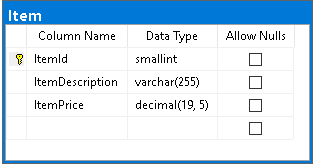
\includegraphics{Images/Item_Table.png}
                \end{center}
    \newpage
    \section{Base Analysis}
    \label{sec:BA}
        \subsection{Raw Results}

    \newpage
    \section{Executive Summary}

    \newpage
    \section{Assumptions}

    \newpage
    \begin{thebibliography}{9}
        \raggedright
        \bibitem{MoneyIssues}
            Reasons against TSQL Money type: Stackoverflow User; \textit{SQLMenace}
            \url{https://stackoverflow.com/questions/582797/should-you-choose-the-money-or-decimalx-y-datatypes-in-sql-server}
        \bibitem{Numeric}
            Microsoft TSQL documentation of Decimal/Numeric types
            \url{https://docs.microsoft.com/en-us/sql/t-sql/data-types/decimal-and-numeric-transact-sql?view=sql-server-2017}
        \bibitem{CTE}
        Microsoft documentation: WITH common\_table\_expression (Transact-SQL)
            \url{https://docs.microsoft.com/en-us/sql/t-sql/queries/with-common-table-expression-transact-sql?view=sql-server-2017}
    \end{thebibliography}

    \newpage
    \section{Appendix}
    \label{sec:Appendix}
    \subsection{CTE Raw Results}
    \label{sec:CTEResults}
    \begin{table}[H]
        \centering
        \begin{tabular}{|l|l|l|}
        \hline
        Reciept\_Id & Customer\_Id & Staff\_Id \\ \hline
        52137       & C27          & S4        \\ \hline
        52137       & C59          & S2        \\ \hline
        52138       & C29          & S13       \\ \hline
        52138       & C30          & S19       \\ \hline
        52139       & C3           & S5        \\ \hline
        52139       & C31          & S20       \\ \hline
        52140       & C38          & S4        \\ \hline
        52140       & C52          & S10       \\ \hline
        52141       & C24          & S19       \\ \hline
        52141       & C42          & S7        \\ \hline
        52142       & C46          & S8        \\ \hline
        52142       & C47          & S6        \\ \hline
        52143       & C51          & S17       \\ \hline
        52143       & C8           & S13       \\ \hline
        52144       & C11          & S10       \\ \hline
        52144       & C50          & S4        \\ \hline
        52145       & C21          & S8        \\ \hline
        52145       & C40          & S15       \\ \hline
        52146       & C38          & S16       \\ \hline
        52146       & C38          & S5        \\ \hline
        52147       & C40          & S18       \\ \hline
        52147       & C9           & S19       \\ \hline
        52148       & C26          & S8        \\ \hline
        52148       & C43          & S16       \\ \hline
        52149       & C10          & S19       \\ \hline
        52149       & C45          & S11       \\ \hline
        52150       & C15          & S10       \\ \hline
        52150       & C57          & S7        \\ \hline
        \end{tabular}
    \end{table}

    \newpage
    \subsection{Python Script}
    \label{sec:Python}

    \newcommand{\includecode}[2][c]{\lstinputlisting[
        language=Python,
        basicstyle=\small,
        caption={Main.py},
        frame=single,
        breaklines=true,
        label=Main Python Script
        commentstyle=\color{blue}
        ]{#2}}

    \begin{center}
        \includecode[width=\textwidth]{Data_Analysis/Scripts/parsedata/main.py}
    \end{center}

    \newpage
    \renewcommand{\includecode}[2][c]{\lstinputlisting[
        language=Python,
        basicstyle=\small,
        caption={Classes.py},
        frame=single,
        breaklines=true,
        label=Main Python Script
        commentstyle=\color{blue}
        ]{#2}}

    \begin{center}
        \includecode[width=\textwidth]{Data_Analysis/Scripts/parsedata/classes.py}
    \end{center}

    
    \end{document}